\documentclass[13pt, letterpaper, twoside]{book}
\usepackage{graphicx}

\usepackage[driver=xetex,paperwidth=8.5in,paperheight=11in,left=1.1in, right=1.74in,top=1.4in, bottom=1.74in]{geometry}
\usepackage[no-math]{fontspec}
\usepackage{newfloat}
\usepackage{sectsty, tikz, color, pgfplots}
\usetikzlibrary{shapes,arrows}
\usepackage{multicol}
\usepackage{amsmath, amssymb, amsfonts,  titlesec}
\usepackage[urw-garamond]{mathdesign}
\usepackage{fancyhdr, booktabs, longtable}
%\usepackage[font=small,format=plain,labelfont=it,textfont=it]{caption}
\usepackage{caption,subcaption}
\usepackage{listings}
\usepackage{algpseudocode, algorithm}
% \usepackage[T1]{fontenc} 
\usepackage{enumitem,verbatim}

 \DeclareTextCommandDefault{\nobreakspace}{\leavevmode\nobreak\ } 

%========== DEFINITIONS ==========

\newlist{alist}{itemize}{1}
\setlist[alist]{label=--,labelindent=2in,leftmargin=9pt,labelsep=6pt, itemsep=0pt}

\def\Lmax{L_{\text{max}}}

%========= FONT SPECS ============
\tolerance 8000

\defaultfontfeatures{Mapping=tex-text, Ligatures=Common}

%\renewcommand\refname{references} % this sets the name of
\def\labelitemi{--}

\def\sansfont{\fontspec[Script=Latin,LetterSpace=2.6, Mapping=tex-text]{DIN 1451 Mittelschrift}}
\def\sansitalicfont{\fontspec[Script=Latin,LetterSpace=2.6, FakeSlant=0.2, Mapping=tex-text]{DIN 1451 Mittelschrift}}

\def\monofont{\fontspec[Script=Latin,Mapping=tex-text,Scale=0.91, AutoFakeBold]{Inconsolata}}

\renewcommand{\texttt}[1]{{\monofont #1}}

%========== COLOR STUFF ===============

\definecolor{darkred}{rgb}{0.6, 0, 0.00}


%============ LISTINGS ==============
\lstset{
aboveskip=2\medskipamount, belowskip=2\medskipamount,
basicstyle=\monofont,
language=python,
numbers=left, numberstyle=\tiny,  numbersep=9pt,
xleftmargin=.4in, frame=l, xrightmargin=1.74in
}


%============= PAGE LAYOUT ============

%\titleformat{\section}{\huge\sansnormalfont}{\protect\makebox[0pt][r]{\thesection\quad}}{0em}{}
\titleformat{\chapter}{\fontsize{32pt}{36pt}\selectfont\sansfont}{}{0em}{}
\titleformat{\section}{\fontsize{18pt}{22pt}\selectfont\sansfont}{\protect\makebox[0pt][r]{\thesection\quad}}{0em}{}
\titleformat{\subsection}{\fontsize{12pt}{16pt}\selectfont\sansfont}{\protect\makebox[0pt][r]{\thesubsection\fontsize{18pt}{22pt}\selectfont\quad}}{0em}{}
%\titleformat{\paragraph}{\fontsize{12pt}{16pt}\selectfont}{}{}{}

\fancyhead[LE]{\sansfont\small An improved batch CP method \normalsize}
\fancyhead[RE]{}
\fancyhead[LO]{}
\fancyhead[RO]{\sansfont\small \nouppercase\rightmark}
\fancyfoot[C]{\sansfont\thepage}

\fancypagestyle{plain}{
\fancyhf{}
\renewcommand{\headrulewidth}{0pt}
\fancyfoot[C]{\sansfont\thepage}
}


\usepackage[pdfpagelayout=TwoPageRight, hidelinks]{hyperref}

\begin{document}
\begin{comment}
\frontmatter

\fontsize{12pt}{16pt}\selectfont
\thispagestyle{empty}
\pagestyle{fancy}

\baselineskip=16.8pt plus 0pt
\frenchspacing

\begin{centering}
\vspace{3em}
\LARGE\sansfont{Scheduling non-identical jobs on a batch resource\\-- Interim
Report --}

\vspace{2em}
\large
\sansfont Sebastian Kosch\\
997 241 024

\vfill
\normalfont
\fontsize{12pt}{16pt}\selectfont
A thesis submitted in conformity with the requirements

for the degree of \textit{Bachelor of Applied Science}

\vspace{1em}
Supervisor: Prof. J. Christopher Beck, MIE

\vspace{2em}

\textmd Division of Engineering Science\\
University of Toronto\\

2013

\end{centering}
\pagebreak

%\include{firstpage}

\tableofcontents
\end{comment}
\pagestyle{fancy}
\mainmatter
\pagebreak
\vskip 4em
\chapter{Introduction}
This paper discusses three different approaches, and several variations on them,
to solving the problem of scheduling non-identical jobs on a batch processing
machine. Batch processing machines, for the purposes of this paper, can process
multiple, non-identical jobs simultaneously -- but all jobs must be loaded into and
unloaded from the machine at once, which introduces a considerable twist on the ``simple
parallel resources'' known from other cases.

The machines in question represents real-life resources like autoclaves or
ovens, which can process multiple items at a time, but often cannot be opened at
random -- in fact, such machines often need to wait for the largest item in the
batch to be done before the next batch can be inserted.

\section{Problem definition}
\section{Organization of this paper}

\chapter{Literature Review}
\section{General MIP and CP}
  \begin{alist}
    \item{Who are the "founders" of MIP and CP?}
    \item{HP Williams}
    \item{Benders}
  \end{alist}
\section{Batch processing}
\begin{alist}
    \item{Azizoglu}
    \item{Dupont}
    \item{Sabouni}
    \end{alist}
\subsection{MIP}
\begin{alist}
    \item{Grossmann}
    \end{alist}
\subsection{CP}
\begin{alist}
    \item{Baptiste}
    \item{Malapert (how does he fit into the picture?)}
\end{alist}
\chapter{Modelling the problem}
\section{Bounds on variables known a priori}

\subsection[Lower bound on $\Lmax$]{Lower bound on {\sansitalicfont L}\textsubscript{max}}
A lower bound on $\Lmax$ can be found using the lower bound on the completion
date of each bucket $q$, where a bucket is defined as the set of batches with
due date $\delta_q$:
\begin{alignat}{2}
& \Lmax \geq C_{\text{max},q} - \delta_q \quad && \forall q
\end{alignat}
This works because the buckets up to bucket $q$ are guaranteed to contain all
jobs with due dates $d \leq \delta_q$, since the batches within the buckets are
ordered by earliest due date (EDD) in the optimal solution. The buckets up to
bucket $q$ will likely also contain some later ($d > \delta_q$) jobs in the
optimal solution but this does not affect the validity of the lower bound.

%To find a lower bound on $C_{\text{max},q}$, we can exploit the fact that every
%batch needs to span its jobs. If we order the jobs up to bucket $q$ by non-increasing processing
%time $p$, then we can use algorithm \ref{alg:findcmax} to find
%$C_{\text{max},q}$:
%\begin{algorithm}
%\begin{algorithmic}
%\State $J^{\star} \gets J$ \Comment{initialize all jobs as unassigned jobs}
%\State $n_k \gets 1$; $S_k \gets \{0\}$; $P_k \gets \{0\}$ \Comment{Create one
%empty batch of size and length zero}
%\State sort $J^{\star}$ by processing time, non-increasing
%\Repeat
%  \State $j \gets J^{\star}$.pop() \Comment{select job for assignment, longest job
%first}
%  \Loop $\;$ through all $n_k$ existing batches $k$, first batch first
%    \State $k_p \gets \emptyset$ \Comment{no feasible batch}
%    \State $c_\text{min} = b$ \Comment{currently known minimum remaining
%    capacity}
%    \If{$s_j < b-S_k$ and $b-S_k < c_\text{min}$}
%      \State $k_p \gets k_p$; $c_\text{min} \gets b-S_k$
%    \EndIf
%  \EndLoop
%  \If{$|k_p| = 1$}
%      \State $S_{k_p} \gets S_{k_p} + s_j$ \Comment{assign job $j$ to batch $k_p$}
%  \Else
%    \State $n_k \gets n_k + 1$\Comment{open new batch}
%    \State $S_{n_k} \gets s_j$; $P_{n_k} \gets p_j$ \Comment{assign $s_j$ and $p_j$ to the new batch}
%  \EndIf
%\Until{$J^{\star}$ is empty}
%\end{algorithmic}
%\caption{Finding $C_{\text{max},q}$}
%\label{alg:findcmax}
%\end{algorithm}
%
%The algorithm is based on the following reasoning: no matter the assignment, one
%batch will have the length $P_k$ of the longest job $\max(p_j)$.
%Since we ordered and assigned the jobs by $p_j$, this will be the first batch
%$k_1$.
%Continue filling $k_1$ until some job $j_c$ exceeds capacity. This job
%must go into another batch $k_2$. Swapping $j_l$ with any of the already assigned jobs
%in $k_1$ (capacity allowing) increases $C_\text{max}$. Even if ``leaving
%capacity'' in $k_1$ for later, better-fitting open jobs may seem desirable --
%these other open jobs will necessarily be shorter than $j_c$, so such a move
%will again serve to increase $C_\text{max}$. Open jobs that fit into
%previous batches with some remaining capacity should be assigned to the batch
%with the \textit{minimum} feasible remaining capacity $c_\text{min}$. This
%avoids unnecessarily precluding shorter (still open) but slightly larger jobs
%from being assigned to previous batches wherever possible. 
%
%A combination of shorter jobs may be a better fit to a previous batch than a
%single, longer job in terms of using remaining capacity, but what matters is
%only the processing time.
%

Now we need to find $C_{\text{max},q}$, or at least a lower bound on it, in
polynomial time. The simplest approach simply considers the ``total elastic area'',
i.e. the sum of all $s_j p_j$ products:
\begin{alignat}{2}
& C_{\text{max},q} \geq \big\lceil\frac{1}{b} \sum_{j} s_j
p_j\big\rceil \quad
&& \forall q, \forall \{ j \in J | d_j \leq \delta_q \}
\end{alignat}
A better lower bound on $C_{\text{max},q}$ would be given by a
preemptive-cumulative schedule. Unfortunately, minimizing $C_{\text{max}}$ for
such problems is equivalent to solving a standard bin-packing problem, which
requires exponential time. 

\subsection[Upper bound on $\Lmax$]{Upper bound on {\sansitalicfont L}\textsubscript{max}}
An upper bound on $\Lmax$ can be found by using a dispatch rule to find a
feasible, if not optimal, schedule. A good approach could be the ``best-fit''
heuristic proposed in the original paper. {\color{darkred} This has not been
implemented yet.}

\subsection[Bounding the number of batches $n_k$]{Bounding the number of batches \sansitalicfont n\textsubscript{k}}
Initially, the number of batches needed is assumed to be equal to the number of
jobs: $n_k = n_j$. Reducing $n_k$ by pre-computing the maximum number of batches
needed shrinks the $x_{jk}$ matrix, and prunes potential search branches in
branch-and-bound decomposition approaches.


\begin{figure}
  \centering
  \begin{subfigure}[b]{0.4\textwidth}
    \centering
    \begin{tikzpicture}[scale=0.2, font=\scriptsize]

      \draw [<->,thick] (0,12) node (yaxis) [above] {\sansitalicfont s}
        |- (25,0) node (xaxis) [right] {\sansitalicfont t};
      \draw[dotted] (0,10) -- (25,10);
        \draw (0,0) rectangle (5,7) node[fn] {$p = 10$\\$d = 10$\\$L = 0$};
        \draw (5,0) rectangle (20, 3) node[fn] {$p = 30, d=20, L=10$};
        
    \end{tikzpicture}
  \end{subfigure}
  \begin{subfigure}[b]{0.4\textwidth}
    \centering
    \begin{tikzpicture}[scale=0.2, font=\scriptsize]

      \draw [<->,thick] (0,12) node (yaxis) [above] {\sansitalicfont s}
        |- (25,0) node (xaxis) [right] {\sansitalicfont t};
      \draw[dotted] (0,10) -- (25,10);
        \draw (0,0) rectangle (5,7) node[fn] {$p = 10$\\$d = 10$\\$L = 20$};
        \draw (0,7) rectangle (15, 10) node[fn] {$p = 30, d=20, L=0$};
    
    \end{tikzpicture}
  \end{subfigure}
\caption{Overzealous batch elimination can increase $\Lmax$}\label{fig:bnk1}
\end{figure}

Unfortunately, we cannot make a general statement that optimal solutions never have more batches than other feasible solutions -- a simple counterexample is shown in figure \ref{fig:bnk1}.\footnote{To be more precise, we cannot state that at least one optimal solution is in the subset of feasible solutions that uses the fewest number of batches -- a dominance situation that could be exploited, were it true.}

Starting out with a one-job-per-batch schedule sorted by EDD, we can explore
all feasible batch configurations recursively. To generate any other feasible
schedule (including the optimal solution), jobs $j$ are rescheduled (``moved back'')
from their original batch $k_\text{origin}$ into a prior batch
$k_\text{earlier}$. This eliminates $k_\text{origin}$ and requires, of course,
that $k_\text{earlier}$ has sufficient capacity. If the job's processing time
$p_j$ exceeds that of $k_\text{earlier}$, then the lateness of batches between
$k_\text{earlier}$ and $k_\text{origin}$ will increase; the merit of such a move
cannot be judged in prior, so it is an \textit{unsafe} batch elimination.
\textit{Safe} eliminations, on the other hand, will never worsen $\Lmax$, and
only they can be considered when bounding $n_k$ a priori.

Algorithm \ref{alg:bounding_nk} outlines a recursive method to find an upper
bound on $n_k$, recognizing safe batch eliminations only.

\begin{algorithm}[h]
\fontsize{9pt}{11.5pt}\selectfont
\begin{algorithmic}
\If{no open jobs left} \Comment{if this is a ``leaf node'' in the recursion}
  \State update UB$(n_k)$
\EndIf
\State find the combination of unsafe later jobs that fills up the capacity
most, leaving us with capacity $b_r$ 
\State find all combinations $x$ of safe later jobs that fit into $b_r$
\Repeat
  \State $x$ = next safe job combination
  \State \textit{ignoreJobs} $\gets x$ \Comment{make the moves, let the next recursion
  level deal with the rest of the jobs}
  \State spawn and run child node with $J \setminus$ \textit{ignoreJobs}
  \State \textit{ignoreJobs} $\gets$ \textit{ignoreJobs} $\setminus x$
\Until{all combinations have been explored}
\State return
\end{algorithmic}
\caption{Recursive algorithm to find an upper bound on $n_k$}
\label{alg:bounding_nk}
\end{algorithm}

This algorithm evidently requires exponential time. A relaxed variant is a
possible option: if only a single unsafe move \textit{into} a batch is possible,
no safe eliminations into that batch are considered at all and we skip to the
next batch. This would greatly speed up the recursion but also significantly
weaken the usefulness of the resulting upper bound.

In a brach-and-bound decomposition approach in which batches are modelled
individually, an upper bound on $n_k$ could be used to limit the depth of the
search tree, or, in combination with a method to determine a lower bound on the
remaining jobs' $n_k$ at every node, to actively prune the search tree during
the search. The latter method, however, would also run in exponential time as
it, again, would require knapsack-type reasoning unless we use a much less powerful
relaxation.

%It is perhaps possible, however, to generate a feasible solution that is likely to use $n_k < n_j$ and to guarantee that such a solution will never use fewer batches than the optimal solution. To do this, let the initial solution $\pi_0$ be a schedule in which every job is assigned to one batch (i.e. $n_k = n_j$) and the jobs are ordered by non-decreasing due date (i.e. $d_n \leq d_{n+1}$), as in figure \ref{fig:bnk2}.
%
%\input{figure showing all the jobs in EDD sequence}
%
%Capacity permitting, jobs are now moved into earlier batches to improve the schedule, eliminating the batch they were placed in initially. Every such move reduces $n_k$ by one.
%
%Two types of moves are possible: \textit{safe} moves and \textit{risky} moves. A move is safe when a job is moved into an earlier batch of longer processing time. A move is risky when a job is moved into an earlier batch of shorter processing time, thus increasing the lateness of that batch.
%
%Moving a job has three effects: 
%
%\begin{alist}
%\item{Effect on the batches after}
%\item{Effect on the batches between, including the new job}
%\item{Effect on the job itself}
%\end{alist}
%
%\begin{table}
%\centering
%\begin{tabular}{r c c}
%\toprule
%              & safe                 & risky \\
%\midrule
%batches after & lateness improves by $p_j$ & lateness improves by $p_a$ \\
%batches between & --- & lateness worsens by $p_j - p_a$ \\
%job itself & lateness improves & lateness improves\\ 
%\bottomrule
%\end{tabular}
%\caption{Lateness effects of safe and risky moves}
%\end{table}
%
%We can easily generate a solution that only contains safe moves.
%We now need to prove that our relaxed solution $\pi_{\text{edd}}$ will never use fewer batches than the optimal solution $\pi_{\text{opt}}$.
%
%For this to be true, we need to show that if there is ever a situation in which we could \textit{either} make $n$ unsafe moves \textit{or} $m>n$ safe ones, using the unsafe ones will never be beneficial if the remaining $m-n$ safe candidates cannot be moved somewhere else.
%
%We're trying to find a relaxation of the problem that is guaranteed to generate as least as many batches as the optimal solution.
%
%
%Whenever there is an alternative between $n$ unsafe moves and $>n$ safe ones, perform $n$ safe ones. Whenever only an unsafe is available, eliminate none and proceed to the next batch.
%
%Unfortunately, we cannot generally state that optimal solutions never have more batches than other feasible solutions: when a job $j_b$ is moved into a prior batch holding $j_a$ and $d_b > d_a$ as well as $p_a < p_b$, it can sometimes happen that $\Lmax$ is increased.
%
%\subsubsection{Some stuff to try}
%
%We can try only considering jobs \textit{before} $\Lmax$, because anything after that job wouldn't be moved in an optimal solution. 
%
%

\begin{comment}
Certain things:
\begin{alist}
\item{When a safe and an unsafe host are available, and we are the last guest,
and the safe host is before the unsafe one, always choose the safe host. (Is this
only true for the last guest?)}
\item{Not moving a job back means it must become a host itself.}
\end{alist}

Open questions: 
\begin{alist}
\item{A job's lateness can only worsen by $p_j$ at a time. Thus, performing safe
elimination on any $\Lmax$ job will make the new host the new $\Lmax$. Is this
true? What implication does that have on what the final schedule looks like?}

\end{alist}
\end{comment}


\section{MIP model}
Malapert's original MIP approach, as given in Model \ref{model:malapertmip},
uses a set of binary decision variables $x_{jk}$ to represent whether job $j$ is
assigned to batch $k$. The original model assumes a set $K$ of $|K| = |J|$
batches, the number of jobs being a trivial upper bound on the number of
batches required; it also enforces an earliest-due-date-first (EDD) ordering of
the batches (constraint \ref{c:malapp-edd}).

\begin{model}[h]
\begin{alignat}{2}
\mathrm{Min.}\quad & \Lmax && \\
\mathrm{s.t.}\quad &\sum_{k \in K} x_{jk} = 1 \quad && \forall j \in J \\
  &\sum_{j \in J} s_j x_{jk} \leq b \quad && \forall k \in K\\
  &p_j x_{jk} \leq P_k \quad && \forall j \in J, \forall k \in K\\
  &C_{k-1} + P_{k} = C_k \quad && \forall k \in K\\
  &(d_{max} - d_j)(1 - x_{jk}) + d_j \geq D_k \quad && \forall j \in J, \forall k \in K\\
  &D_{k-1} \leq D_k \quad && \forall k \in K \label{c:malapp-edd} \\
  &C_k - D_k \leq \Lmax \quad && \forall k \in K\\[2ex]
  &C_k \geq 0, P_k \geq 0 \text{ and } D_k \geq 0 \quad && \forall k \in K  
\end{alignat}
\caption{Malapert's original MIP model}
\label{model:malapertmip}
\end{model}

\section{Improved MIP model}
Several improvements can be made to Malapert's MIP model in the form of
additional constraints shown in Model \ref{model:improvedmip}, as  
described in greater detail in the subsections below.

\begin{model}[h]
\begin{alignat}{2}
& \sum_{j \in J} x_{j,k-1} = 0 \rightarrow \sum_{j \in J} x_{jk} = 0 \quad &&
\forall k \in K \\
& e_k + \sum_{j \in J} x_{jk} \geq 1 \quad && \forall k \in K \\
& n_j (e_k-1) + \sum_{j \in J} x_{jk} \leq 0 \quad && \forall k \in K \\
& e_k - e_{k-1} \geq 0 \quad && \forall k \in K \\
& x_{jk} = 0 \quad && \forall \{j \in J, k \in K | j > k \} \\
& \Lmax \geq \big\lceil\frac{1}{b} \sum_{j} s_j
p_j\big\rceil - \delta_q \quad
&& \forall q, \forall \{ j \in J | d_j \leq \delta_q \}
\end{alignat}
\caption{Improvements to Malapert's original MIP model}
\label{model:improvedmip}
\end{model}

\subsection{Grouping empty batches} The given
formulation lacks a rule that ensures that no empty batch is followed by a
non-empty batch. Empty batches have no processing time and a due date only
bounded by $d_\text{max}$, so they can be sequenced between non-empty batches
without negatively affecting $\Lmax$. Since, however, desirable schedules have
no empty batches scattered throughout, we can easily reduce the search space by
disallowing such arrangements. The idea is illustrated in Figure
\ref{fig:dominancerule}.


\begin{figure}
  \centering
  \begin{subfigure}[b]{0.4\textwidth}
    \centering
    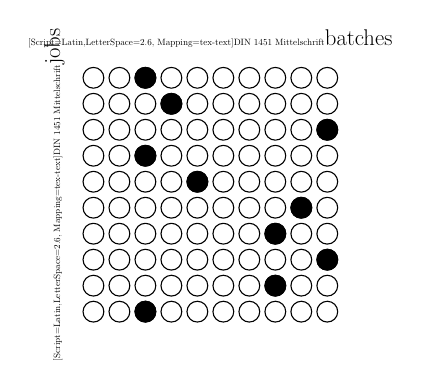
\begin{tikzpicture}[scale=0.33]
      \pgftext[x=-1.5cm, y=4.5cm, rotate=90]{\sansfont\Huge jobs}
      \pgftext[x=4.5cm, y=10.5cm]{\sansfont\Huge batches}

      \foreach \j in {0,...,9}
      {
        \foreach \k in {0,...,9}
        {
          \draw[] (\k, \j) circle [radius=0.4];
        }
      }
      \draw [fill] (2,0) circle [radius=0.4];
      \draw [fill] (2,6) circle [radius=0.4];
      \draw [fill] (2,9) circle [radius=0.4];
      \draw [fill] (3,8) circle [radius=0.4];
      \draw [fill] (4,5) circle [radius=0.4];
      \draw [fill] (7,1) circle [radius=0.4];
      \draw [fill] (7,3) circle [radius=0.4];
      \draw [fill] (8,4) circle [radius=0.4];
      \draw [fill] (9,2) circle [radius=0.4];
      \draw [fill] (9,7) circle [radius=0.4];
    \end{tikzpicture}
    \caption{Without dominance rule}
  \end{subfigure}
  \begin{subfigure}[b]{0.4\textwidth}
    \centering
    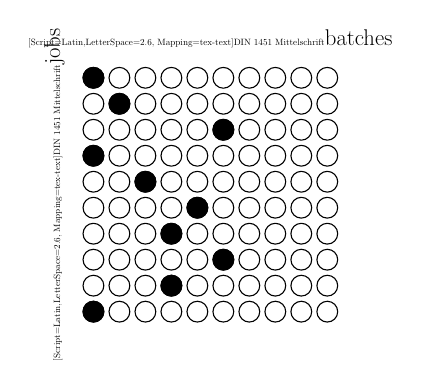
\begin{tikzpicture}[scale=0.33]
      \pgftext[x=-1.5cm, y=4.5cm, rotate=90]{\sansfont\Huge jobs}
      \pgftext[x=4.5cm, y=10.5cm]{\sansfont\Huge batches}

      \foreach \j in {0,...,9}
      {
        \foreach \k in {0,...,9}
        {
          \draw[] (\k, \j) circle [radius=0.4];
        }
      }
      \draw [fill] (0,0) circle [radius=0.4];
      \draw [fill] (0,6) circle [radius=0.4];
      \draw [fill] (0,9) circle [radius=0.4];
      \draw [fill] (1,8) circle [radius=0.4];
      \draw [fill] (2,5) circle [radius=0.4];
      \draw [fill] (3,1) circle [radius=0.4];
      \draw [fill] (3,3) circle [radius=0.4];
      \draw [fill] (4,4) circle [radius=0.4];
      \draw [fill] (5,2) circle [radius=0.4];
      \draw [fill] (5,7) circle [radius=0.4];
    \end{tikzpicture}
    \caption{With dominance rule}
  \end{subfigure}
\caption{Dominance rule to eliminate empty batches followed by non-empty batches
(circles represent the $x_{jk}$ variables; a filled circle stands for $x_{jk} =
1$)}\label{fig:dominancerule}
\end{figure}


A mathematical formulation is
\begin{alignat}{2}
& \sum_{j \in J} x_{j,k-1} = 0 \rightarrow \sum_{j \in J} x_{jk} = 0 \quad && \forall k \in K. \label{eq:emptybatch0}
\end{alignat}

To implement this, we can write constraints in terms of an additional  set of binary variables, $e_k$, indicating whether a batch $k$ is empty or not:

\begin{alignat}{2}
& e_k + \sum_{j \in J} x_{jk} \geq 1 \quad && \forall k \in K, \label{eq:emptybatch1} \\
& n_j (e_k-1) + \sum_{j \in J} x_{jk} \leq 0 \quad && \forall k \in K. \label{eq:emptybatch2}
\end{alignat}

Constraints \eqref{eq:emptybatch1} enforce $e_k = 1$ when the batch $k$ is
empty. Constraints \eqref{eq:emptybatch2} enforce $e_k = 0$ otherwise, since the sum term will never exceed $n_j$. The rule \ref{eq:emptybatch0} can now be expressed as $e_{k-1} = 1 \rightarrow e_k = 1$, and implemented as follows:

\begin{alignat}{2}
& e_k - e_{k-1} \geq 0 \quad && \forall k \in K.
\end{alignat}

We can also prune any attempts to leave the first batch empty by adding a constraint $e_0 = 0$.


\subsection{No postponing of jobs to later batches}
Since the jobs are already sorted by non-decreasing due dates, it makes sense to explicitly instruct the solver never to attempt to push jobs into batches with a greater index than their own: even if every job had its own batch, it would be unreasonable to ever postpone a job to a later batch.
\begin{alignat}{2}
  & x_{jk} = 0 \quad && \forall \{j \in J, k \in K | j > k \}
\end{alignat}

\subsection[Lower bound on $\Lmax$]{Lower bound on {\sansitalicfont L}\textsubscript{max}}
Let a \textit{bucket} $q$ denote the set of all batches with due date $\delta_q$.
Then the completion date $C_q$ of this bucket is the completion date of the
last-scheduled batch with due date $\delta_q$, and the lateness of the bucket
$q$ is $L_q = C_q - \delta_q$. Since all batches up to and including those in
bucket $q$ are guaranteed to contain all jobs with due dates $d \leq \delta_q$
-- as ensured by the EDD ordering of batches -- the lower bound on every
bucket's lateness $LB(L_q)$ is a valid lower bound on $\Lmax$. In other words,
jobs with due date $d \leq \delta_q$ will be found only in batches up to and
including the last
batch of bucket $q$. This provides a lower bound on the lateness of bucket $q$:
\begin{alignat}{2}
& \Lmax \geq C_{\text{max},q} - \delta_q \quad && \forall q
\end{alignat}
The buckets up to bucket $q$ will likely also contain some later ($d >
\delta_q$) jobs in the optimal solution but this does not affect the validity of
the lower bound.

Now we need to find $C_{\text{max},q}$, or at least a lower bound on it, in
polynomial time. The simplest approach simply considers the jobs' total ``area''
(or ``energy''), i.e. the sum of all $s_j p_j$ products:
\begin{alignat}{2}
& C_{\text{max},q} \geq \big\lceil\frac{1}{b} \sum_{j} s_j
p_j\big\rceil \quad
&& \forall q, \forall \{ j \in J | d_j \leq \delta_q \}
\end{alignat}
A better lower bound on $C_{\text{max},q}$ would be given by a
preemptive-cumulative schedule. Unfortunately, minimizing $C_{\text{max}}$ for
such problems is equivalent to solving a standard bin-packing problem, which
requires exponential time.\footnote{In a preemptive-cumulative schedule, jobs
may be stopped and restarted mid-execution, but occupy a constant amount $s_j$
on the resource while executing. In such a schedule, minimizing the makespan is
as difficult as solving a bin-packing problem: we can break jobs into small
pieces (no longer than the smallest common divisor of the jobs' lengths $p$) and
then pack them together such as to minimize the number of small time slots
needed.}



\section{CP model}

The mixed integer model can be turned into a constraint programming model with
just a small number of modifications.

\subsection{Bin-packing and cumulative constraints} This makes sure the jobs are
distributed into the batches such that no batch exceeds the capacity $b$:
\begin{align} \mathtt{pack}(J, K, b) \end{align}

The cumulative constraint functions similarly, but instead of packing discrete
bins, it enforces non-overlapping constraint on the temporal
(\texttt{IntervalVariable}) $J$ variables.  \begin{align} \mathtt{cumul}(J, b)
\end{align}

\subsection{Temporal constraints} These constraints are implemented using
\texttt{IntervalVar} objects, which offer properties such as \texttt{lengthOf}
or \texttt{endOf}.

\begin{alignat}{2} & P_k \geq \underset{j : B_j = k}{\max} \; p_j \quad &&
\forall k \in K \\ & D_k \leq \underset{j : B_j = k}{\min}\; d_j \quad &&
\forall k \in K \\ & C_k + P_{k+1} = C_{k+1} \quad && \forall k \in K \\ & \Lmax
\geq \underset{k}{\max} \;(C_k - D_k) && \end{alignat}

The first constraint ensures that each batch is as long as its longest job.  The
second constraint ensures that the earliest-due job sets the due date.  The
third constraint defines batch completion dates, and the fourth constraint
defines $\Lmax$.

The first two temporal constraints exploit the temporal features of
\texttt{IntervalVar}s.

\subsection[Constraint on the number of batches with length $P_k >
p$]{Constraint on number of batches with length {\sansitalicfont
P\textsubscript{k}} > {\sansitalicfont p}}

Since batches take on the processing time of their longest job, there is at
least one batch with $P = \underset{j}{\max} p_j $: \begin{align}
\mathtt{globalCardinality}( |P_k = \underset{j}{\max} \; p_j| = 1 ) \end{align}
We can proceed to fill batches with jobs, ordered by non-increasing processing
time, based on algorithm \ref{alg:findBatchlengthCards}. 

\begin{algorithm}[h!]
\fontsize{9pt}{11.5pt}\selectfont \begin{algorithmic} \State $J^{\star} \gets J$
\Comment{initialize all jobs as unassigned jobs} \State $n_k \gets 1$; $S_k
\gets \{0\}$; $P_{k,\text{min}} \gets \{0\}$ \Comment{Create one empty batch of
size and length zero} \State sort $J^{\star}$ by processing time, non-increasing
\Repeat \State $j \gets J^{\star}$.pop() \Comment{select job for assignment,
longest job first} \Loop $\;$ through all $n_k$ existing batches $k$, first
batch first \State $k_p \gets \emptyset$ \Comment{no feasible batch} \State
$c_\text{min} = b$ \Comment{currently known minimum remaining capacity} \If{$s_j
< b-S_k$ and $b-S_k < c_\text{min}$} \State $k_p \gets k_p$; $c_\text{min} \gets
b-S_k$ \EndIf \EndLoop \If{$|k_p| = 1$} \State $S_{k_p} \gets S_{k_p} + s_j$
\Comment{assign job $j$ to batch $k_p$} \Else \If{$n_k < LB(n_k)$} \State $n_k
\gets n_k + 1$\Comment{open new batch} \State $S_{n_k} \gets s_j$;
$P_{n_k,\text{min}} \gets p_j$ \Comment{assign $s_j$ and $p_j$ to the new batch}
\Else \State leave the loop now and end.  \EndIf \EndIf \Until{$J^{\star}$ is
empty} \end{algorithmic} \caption{Generating lower bounds on batch lengths}
\label{alg:findBatchlengthCards} \end{algorithm}
At the end of this algorithm, we can state: \begin{alignat}{2} &
\mathtt{globalCardinality}( |P_{k-1,\text{min}} > P_k \geq P_{k,\text{min}} |
\geq 1) \quad && \forall k \in \{k_0,\dots,k_{LB(n_k)}\} \end{alignat}

The algorithm sorts jobs by non-increasing $p$, and then fills batches job by
job. If a job fits into a previous batch, it is assigned there. If a job fits
into multiple previous batches, it is assigned to the batch with the smallest
remaining capacity. This is sometimes called \textit{best-fit dereasing} rule,
and works as follows: let $J^\star$ be the set of jobs sorted by $p$, then at
least one batch will be as long as the longest job $j^\star_1$. If the next $n$
jobs fit into this batch, then there is at least one batch not shorter than
$j^\star_{n+1}$, and similarly for subsequent batches. 
{\color{darkred} 
Unfortunately, optimal solution may perform better than the packing heuristic in
terms of ``vertical'' ($s_j$) bin packing, and may thus require fewer batches.
We therefore need to find a lower bound $LB(n_k)$ on the number of batches, and
we can only guarantee the first $LB(n_k)$ of the above constraints to hold in
the optimal solution. Finding a true lower bound is a two-dimensional bin
packing problem, which runs in exponential time $\dots$ so we
have to come up with an even lower bound -- right now I can only think of $j_0$,
the number of jobs ordered by decreasing $s_j$ that can never fit into a batch
together.}

Furthermore, if all jobs have different processing times, all batches will have
different processing times as well: \texttt{alldifferent}$(P_k)$. If $m$ out of
$n_j$ jobs have different processing times, we can still enforce
\texttt{k\_alldifferent}$(P_k, m)$.  Propagation rules for this constraint were
given in \cite{Lardeux}.  {\color{darkred} I can't find anything on this w.r.t.
CP Optimizer, so I may have to implement this myself $\dots$ time permitting.} 

\subsection{Temporal constraints on a job's start date} Given any partial
assignment of jobs and an open job $j$, we can reason that \begin{alist}
\item{if the first batch with a due date later than the job is $k$, then the job
cannot be part of a batch after $k$ -- this would result in a non-EDD sequence
of batches.} \item{if the first batches up to $k-1$ offer not enough capacity
for $j$ due to the given partial assignment, then the job cannot be part of a
batch before $k$.} \end{alist} Since batches are \textit{not} dynamically
created like in Malapert's solution but fixed from the start, any partial
assignment that fails due to these constraints cannot be part of an optimal
solution.

This constraint is redundant with both the $(C_{k+1}\geq C_k)$ and
\texttt{packing} constraints, but may help accelerate the propagation in some
cases.

\subsection{Grouping empty batches} Just like in the MIP model, we can force
empty batches to the back and thus establish dominance of certain solutions. The
implementation is much easier than in the MIP model: \begin{alignat}{2} &
\mathtt{IfThen}( C_{k+2} > C_{k}, C_{k+1} > C_{k} ) \quad && \forall k \in
\{k_1, \dots, k_{n_k-2}\} \end{alignat}

\subsection{No postponing of jobs to later batches} Just like in the MIP model,
jobs should never go into a batch with an index greater than their own:
\begin{alignat}{2} & x_{jk} = 0 \quad && \forall j,k : j > k \end{alignat} This
is implemented as $\mathtt{assignments}_j \leq k$. 

{\color{darkred} This constraint is analogous to the concept of finding an upper
bound on $n_k$ -- essentially, it would be very helpful to find an upper bound
on the latest batch for \textit{every} job.}



\section{Decomposition approach}

Instead of solving the entire problem using one model, we can solve the problem
step by step, using the best techiques available for each subproblem. This
approach is inspired by a method called \textit{Benders' decomposition}.

\subsection{Branch-and-bound by batch in chronological order}
A basic version of this approach uses branch-and-bound to transverse the search
tree. At each node on level $\ell$, a single MIP and/or CP model is run to
assign jobs to batch $k = \ell$. The remaining jobs are passed to the children
nodes, which assign jobs to the next batch, and so on -- until a solution, and
thus a new upper bound on $\Lmax$, is found. Several constraints are used to
prune parts of the search tree that are known to offer only solutions worse than
this upper bound. Figure \ref{fig:decomp_diagram1} shows an example in which a
MIP model is used to assign jobs to the batch at every node.
\begin{algorithm}[h]
\fontsize{9pt}{11.5pt}\selectfont
\begin{algorithmic}
\State update \textit{currentAssignments} \Comment{this keeps track of where we are
in the tree}
\If{no jobs given to this node} \Comment{if this is a leaf node, i.e. all jobs
are assigned to batches}
  \State calculate $L_{\text{max,current}}$ based on \textit{currentAssignments}
  \If{$L_{\text{max,current}}$ < $L_{\text{max,incumbent}}$}
    \State $L_{\text{max,incumbent}} \gets L_{\text{max,current}}$
    \State \textit{bestAssignments} $\gets$ \textit{currentAssignments}
  \EndIf
  \State return to parent node
\EndIf
\State set up MIP model \Comment{as described below}
\Repeat
  \State $x_j \gets$ model.solve($x_j$) \Comment{let model assign jobs to the
  batch}
  \State spawn and run child node with all $\{j | x_j = 0\}$ \Comment{pass
  unassigned jobs to children}
  \State add constraint to keep this solution from recurring \Comment{this
  happens once the child node returns}
\Until{model has no more solutions}
\State return to parent node
\end{algorithmic}
\caption{MIP node class code overview}
\label{alg:bbnode_mip1}
\end{algorithm}
Algorithm \ref{alg:bbnode_mip1} outlines what happens at each node: the model
finds the best jobs to assign to the batch according to some rule, lets the
children handle the remaining jobs, and tries the next best solution once the
first child has explored its subtree and backtracked.
\subsubsection{Using MIP and cumulative packing after the batch}
\tikzset{
  treenode/.style = {align=center, inner sep=4pt, text centered,
    font=\sansfont\fontsize{11pt}{12pt}\selectfont},
  root/.style = {treenode},% arbre rouge noir, noeud noir
  nchild/.style = {treenode,
     },% arbre rouge noir, noeud rouge
  leaf/.style = {treenode}% arbre rouge noir, nil
}

\begin{figure}
\centering
\begin{tikzpicture}[->,>=stealth',level/.style={sibling distance = 3cm/#1,
  level distance = 1.5cm}, scale=0.7]
\node (Root) [root] {MIP}
 child{ node [nchild] {MIP} 
            child{ node [nchild] {MIP}}
            child{ node [nchild] {MIP}
              child{ node [leaf] {Solution 1}}
						}                            
    }
    child{ node [nchild] {MIP} }
    child{ node [nchild] {MIP} 
            child{ node [nchild] {MIP} %2, left
                    child{ node [leaf] {Solution 2}} 
                  }
            child{ node [nchild] {MIP} }
		};
  \begin{scope}[every node/.style={right}]
    \path (Root -| Root-3-2) ++(1.5cm,0) node {\fontsize{10pt}{10pt}\selectfont $k=1$};
    \path (Root-1 -| Root-3-2) ++(1.5cm,0) node
    {\fontsize{10pt}{10pt}\selectfont $k=2$};
    \path (Root-1-1 -| Root-3-2) ++(1.5cm,0) node
    {\fontsize{10pt}{10pt}\selectfont $k=3$};
  \end{scope}

   \end{tikzpicture}
\caption{Batch-by-batch decomposition using MIP only}\label{fig:decomp_diagram1}
\end{figure}

The first version of the branch-and-bound batch-by-batch decomposition uses a
MIP model at each node to assign jobs to the respective batch. The remaining
jobs are packed such as to minimize their $\Lmax$, with a relaxation of the
batching requirement, i.e., as if on a cumulative resource. 
\begin{model}[h!]
\begin{alignat}{3}
\text{Min.}\quad & L_{\text{max,cumul}} && \\ 
\text{s. t.}\quad & \label{dc:eq1} \sum_j s_j x_j \leq b \quad && \forall j \in J \\
& P_k \geq p_j x_j \quad && \forall j \in J \\
& \label{dc:eq3} \sum_j x_j \geq 1 \quad && \forall \{j \in J | d_j = \min(d_j)\} \\
& \label{dc:eq4} P_k + \frac{1}{b} \sum_{i} s_i p_i \leq d_j +
L_{\text{max,incmb}} - 1 - v_k \quad && \forall j \in J, \forall \{i \in J | d_i
\leq d_j\} \\[2ex]
& \label{dc:eq5} \sum_t u_{jt} = 1 \quad && \forall j \in J \\
& \label{dc:eq6} \sum_j \sum_{t' \in T_{jt}} u_{jt'} \leq b \quad && \forall t \in \mathcal{H} \\
& \label{dc:eq7} (v_k + t + p_j) u_{jt} \leq d_j + L_{\text{max,incmb}} - 1 \quad && \forall j \in J, \forall t \in \mathcal{H} \\
& \label{dc:eq8} L_{\text{max,cumul}} \geq (v_k + t + p_j) u_{jt} - d_j \quad && \forall j \in J, \forall t \in \mathcal{H} \\
& \label{dc:eq9} u_{j,t=1} = x_j \quad && \forall j \in J \\
& \label{dc:eq10} u_{it} \leq (1 - x_j) \quad && \forall i,j \in J, \forall t
\in \mathcal{H} \setminus \{2\} \\[2ex]
& \label{dc:eq11} b - \sum_j s_j x_j \leq (b w_j + 1) s_j \quad && \forall j \in J \\
& \label{dc:eq12} P_k + 2w_j n_t \geq p_j + n_t x_j \quad && \forall j \in J\\
& \label{dc:eq13} P_k - 2(1 - w_j)n_t \leq p_j +n_t x_j - 1 \quad && \forall j
\in J
\end{alignat}
\caption{MIP model in batch-by-batch branch-and-bound}
\label{model:decomp_mip}
\end{model}

\begin{table}[h]
\begin{tabular}{l p{5in}}
$x_j$ & is 1 iff job $j$ is assigned to the batch \\
$u_{jt}$ & is 1 iff job $j$ starts in time slot $t$ \\
$T_{jt}$ & is the set of all time slots occupied by job $j$ if it ended at time
$t$, that is $T_{jt} = \{t - p_j + 1, \dots, t\}$ \\
$v_k$ & is the start time of the batch at the given node in the search tree \\
$L_{\text{max,incmb}}$ & is the incumbent (known best) value of and thus an
upper bound on $\Lmax$ \\
$\mathcal{H}$ & is the set of all indexed time points $\{1, \dots, n_t\}$ \\
$w_j$ & is 1 iff job $j$ is either longer than the batch ($p_j > P_k$) or
already part of the batch ($x_j = 1$)
\end{tabular}
\caption{Notation used in the decomposition model}
\end{table}

Model \ref{model:decomp_mip} implements a time-indexed cumulative constraint on the
non-batched jobs. Constraints \eqref{dc:eq1} through \eqref{dc:eq3} ensure that the
batch stays below capacity, define the duration of the batch $P_k$ and force at
least one of the earliest-due jobs into the batch.

Constraints \eqref{dc:eq4} express the interval relaxation used to ensure that no
jobs exceed their latest allowable finish date given any batch assignment. Even
jobs that are assigned to the batch have to fulfill this requirement.

Constraints \eqref{dc:eq5} and \eqref{dc:eq6} implement the cumulative nature of the
post-batch assignments by ensuring that each job starts only once, and no jobs
overlap on a given resource at any time (for the purposes of this model, the
batch machine is considered divisible into $b$ unary resources).

Constraints \eqref{dc:eq7} again limit the possible end dates of a
job, but unlike \eqref{dc:eq4}, they use the time assignments on the cumulative
resource to determine end dates. Constraints \eqref{dc:eq8} define the value of
$L_{\text{max,cumul}}$, the maximum lateness of any job in the non-batched set.

Constraints \eqref{dc:eq9} force batched jobs to start at $t = 0$, while \eqref{dc:eq10} force \textit{all} jobs to start either at $t = 0$ or after the last batched job ends.

Constraints \eqref{dc:eq11} enforce a dominance rule: jobs must be assigned to
the batch such that the remaining capacity, $b_r = b - \sum_j s_j x_j$, is less than
the size $s_j$ of the \textit{smallest} job from the set of non-batched jobs that
are \textit{not longer} than the current batch. That is, if there exists an
non-batched job $j$ with $p_j \leq P_k$ and $s_j \leq b_r$, then the current
assignment of jobs is infeasible in the model. The reasoning goes as follows:
given any feasible schedule, assume there is a batch $k_a$ with $b_r$ remaining capacity
and a later batch $k_b$ containing a job $j$ such that $s_j \leq b_r$ and $p_j \leq
P_{k_a}$. Then job $j$ can always be moved to batch $k_a$ without negatively affecting the
quality of the solution: if the schedule was optimal, then moving $j$ will not
affect $\Lmax$ at all (otherwise, it was no optimal schedule); if the schedule
was not optimal, then $\Lmax$ will stay constant (unless $j$ was the longest job
in $k_b$ and $\Lmax$ occured in or in a batch after $k_b$, in which case $\Lmax$ will
be improved).

This rule is implemented by means of a binary variable $w_j$, which, as defined
by constraints \eqref{dc:eq11} and \eqref{dc:eq12}, is 1 iff $p_j > P_k \lor x_j
= 1$. These are the cases in which a job $j$ is \textit{not} to be considered in \eqref{dc:eq10}, and so $w_j$ is used to scale $s_j$ to a value
insignificantly large in the eyes of the constraint's less-than relation.

After a solution is found, a child node in the search tree has run the subtree
and returned, a constraint of the form 
\begin{alignat}{2}
& \sum_j x_j + \sum_i (1-x_i) \leq n_j - 1 \quad && \forall \{j \in J | x_j =
1\}, \forall \{i \in J | x_i = 0 \}
\end{alignat}
is added to the model before the solver is called again, to exclude the last
solution from the set of feasible solutions. 

\subsubsection{Using CP and cumulative packing after the batch}
This approach is equivalent, but we now use CP to select the batch assignments,
again based on a minimized $\Lmax$ among the non-batched jobs. 

\begin{model}[h]
\begin{alignat}{2}
\mathrm{Min.} \quad & \Lmax \quad && \\
\mathrm{s.t.} \quad & \mathtt{IfThen}(x_j = 0, \startOf(j) \geq P_k) \quad && \forall j
\in J \\
& \mathtt{IfThen}(\startOf(j) \geq 2, x_j = 0) \quad && \forall j \in J \\
& \mathtt{IfThen}(x_j = 1, \startOf(j) = 0) \quad && \forall j \in J \\
& \mathtt{IfThen}(\startOf(j) = 1, x_j = 1) \quad && \forall j \in J \\
& P_k \geq x_j p_j \quad && \forall j \in J \\
& \endOf(j) = d_j + L_{\text{max,incmb}} - 1 \quad && \forall j \in J \\
& \Lmax \geq \endOf(j) - d_j \quad && \forall j \in J \\
& \mathtt{IfThen}(p_j \leq P_k \land x_j = 0, b - \sum_{j \in J} s_j
x_j \leq s_j) \quad && \forall j \in J \\
& P_k + \frac{1}{b} \sum_i s_i p_i \leq d_j + L_{\text{max,incmb}} - 1 - v_k
\quad && \forall j \in J, \forall \{i \in J | d_i \leq d_j\} \\
& \sum_j x_j \geq 1 \quad && \forall \{ j \in J | d_j = \min(d_j) \} \\
& \mathtt{cumul}(J, b) \quad & &  
\end{alignat}
\caption{CP model in batch-by-batch branch-and-bound}
\label{model:decomp_cp}
\end{model}


\subsection{Potential improvements}
\paragraph{Improve the initial $L_{\text{max,incumbent}}$} A better initial
upper bound on $\Lmax$ can help prune some branches of the search tree from the
outset. There are several dispatch rules (or maybe other heuristics?) that could
be explored to do this better.
\paragraph{Improve $L_{\text{max,incumbent}}$ during search} It may be useful to
use a heuristic like above to ``complete the schedule'' once a promising partial
schedule has been generated. I have yet to identify situations where this is
always helpful.




\newpage
\chapter{Results}
\section{Empirical comparison of described models}\label{sec:results}
The models were tested on a set of job lists. Malapert's paper uses benchmark
job lists by \citet{daste1, daste2}. Since neither publication is
available online, I created my own set of randomized job lists for the purposes
of this paper, with $s_j, p_j \in [1, 20]$ and $d_j \in [1, 10n_j]$ where $n_j$ is
the number of jobs.\footnote{These instances will be updated to reflect the
feature distributions used in Daste et al.} Ten different sample job sets are
used per unique value of $n_j$. The times shown in figure \ref{fig:comp_times}
are averaged over those ten instances for each $n_j$.

The models were run on an i7 Q740 CPU in single-thread mode, with 8 GB RAM.
Solving was aborted after a time of 3600 seconds (1 hour).

The CP branch-and-bound model times out on most instances and is not shown here.
The CP model times out on one 12-job instance and gets progressively worse with
more jobs; similar to Malapert's original MIP model.
\begin{figure}
\centering

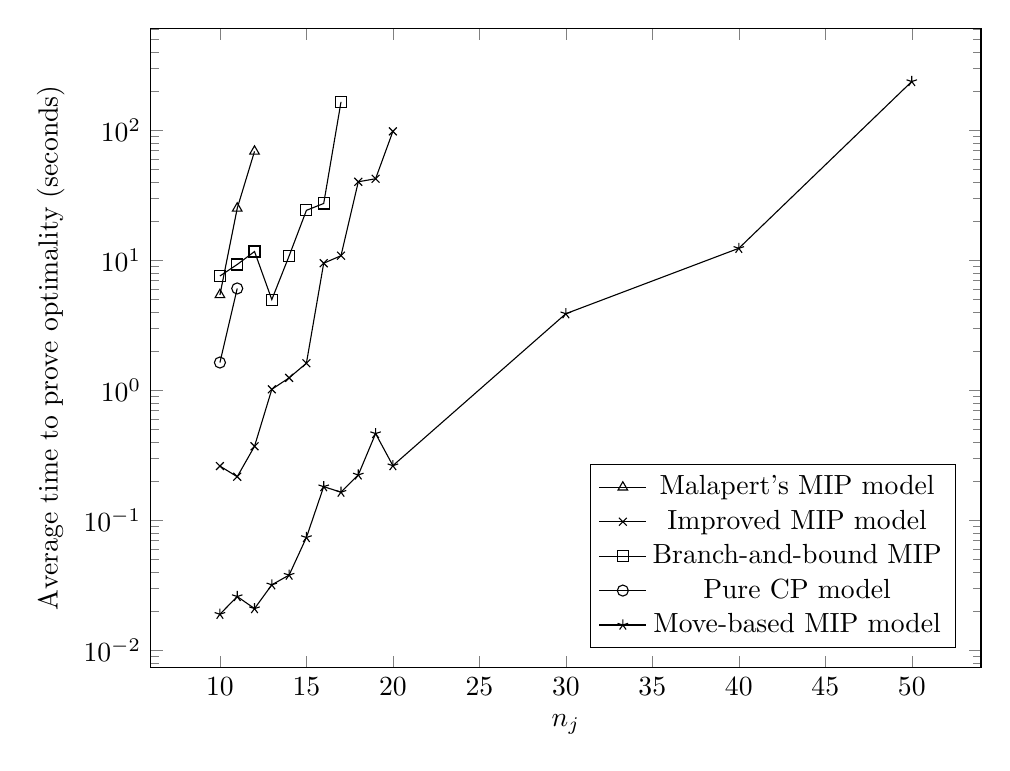
\begin{tikzpicture}
  \begin{semilogyaxis}[xlabel=$n_j$, ylabel=Average time to prove optimality (seconds), width=\textwidth,
  height=0.8\textwidth,legend pos=south east]
  \addplot[color=black, mark=triangle ] coordinates { % MIP model times
  (10, 5.441)
  (11, 25.18)
  (12, 69.05)
  };   \addlegendentry{Malapert's MIP model}

  \addplot[color=black, mark=x ] coordinates { % MIP model times
  (10, 0.262)
  (11, 0.217)
  (12, 0.372)
  (13, 1.02)
  (14, 1.25)
  (15, 1.62)
  (16, 9.52)
  (17, 10.88)
  (18, 40.3)
  (19, 42.5)
  (20, 98.415)
  };   \addlegendentry{Improved MIP model}

  \addplot[color=black, mark=square] coordinates {
(10, 7.59)
(11, 9.31)
(12, 11.72)
(13, 5)
(14, 10.83)
(15, 24.28)
(16, 27.44)
(17, 165.82)
  };
  \addlegendentry{Branch-and-bound MIP}
  \addplot[color=black, mark=o] coordinates {
(10, 1.64)
(11, 6.09)
};
  \addlegendentry{Pure CP model}
  \addplot[color=black, mark=star] coordinates {
(10, 0.019)
(11, 0.026)
(12, 0.021)
(13, 0.032)
(14, 0.038)
(15, 0.074)
(16, 0.182)
(17, 0.165)
(18, 0.224)
(19, 0.466)
(20, 0.264)
(30, 3.895)
(40, 12.403)
(50, 238)
};
  \addlegendentry{Move-based MIP model}
  \end{semilogyaxis}
\end{tikzpicture}

\caption{Comparison of CPU time used by different models to find an optimal
schedule and prove its optimality.}
\label{fig:comp_times}
\end{figure}






\begin{comment}
\chapter{My solution}
\section{MIP formulation improvements}
\section{CP formulation improvements}

\chapter{Discussion}


\pagebreak

\vskip 4em
\end{comment}

\end{document}

